\section{Registration, freeze, data access, and deviations}
\label{app:reg}

\begin{itemize}
  \item \textbf{Registration.} \texttt{prereg/study3/PREREGISTRATION.md} v3, frozen with \texttt{prereg/study3/inputs.sha256} (37 files) in commit \texttt{c8feea1} on 14 October 2026, before any registered game. It was not lodged with any external registry. The frozen document still carries its draft status line (``NOT registered, NOT frozen'') and its plan to record an external registry's timestamp before any game; the freeze commit and the hash check were carried out as written, while the external timestamp was not. The freeze order rests on the local git history (\texttt{c8feea1} at 17:28 MDT, 23:28 UTC) and on the six session manifests, which record the commit each session ran from (\texttt{c8feea1}; for API session 2, \texttt{c2292c1}, which adds only the data-access log) and the hash of every frozen file. The first registered call was sent at 23:54 UTC, 25 minutes after the freeze commit.
  \item \textbf{Decisions before the freeze.} (1) Scripted openings in zone units rather than own-limit gaps, set on 13 October before any game, because transplanted gaps made some scripted pairs cross. (2) Trailing text after the first JSON object is ignored and flagged (14 October, after the first API pilot, which was rerun under it). Luna had \sThreeTrailingLuna{} such replies; no other model had any.
  \item \textbf{Data access.} Logged in \texttt{prereg/study3/DATA\_ACCESS.md}, each entry committed before the look: an interim look at Gemma and Qwen (commit \texttt{c2292c1}) before the second API session, and the single registered analysis of all five models (commit \texttt{8a3167d}).
  \item \textbf{Run incident.} API session 2 stalled when the host machine slept after 1{,}266 games. It was resumed from the same commit; no finished game was replayed and no attempt was voided.
  \item \textbf{Quality.} Counts by model are in Table~\ref{tab:s3-quality}. Luna had \sThreeForfeitsLuna{} forfeits and \sThreeTimeoutsLuna{} timeouts. All three API models had 0 refusals, 0 reasoning tokens, and 0 reasoning text (Gemini included). Returned versions were unchanged across sessions: \texttt{openai/gpt-6-luna-20260922}, \texttt{anthropic/claude-haiku-5.5-20261007}, and \texttt{google/gemini-3.5-flash-lite-20260721}.
  \item \textbf{Cost.} API fees, as OpenRouter reported them, were \$16.96 for the two registered sessions and \$0.56 for the two format pilots. GPU time for Study 3 was about \$10.90 including its pilots, and for E5 and E6 about \$1.62 and \$0.58 (launcher estimates, not billing records).
\end{itemize}

\section{Full Study 3 results}
\label{app:study3-full}

Table~\ref{tab:s3-quality} gives game outcomes and data quality by model. Outside-zone agreements (retained unclipped, as registered) broke down by cell as follows: \textbf{Gemini} (120/3{,}200): A0 9/320 at \$100, 8 at \$100K, 20 at \$100M; A1 38 at \$100, 7 at \$100K, 4 at \$100M; clamp 24 (\texttt{x1e2-o1e2}), 7 (\texttt{x1e2-o1e8}), 3 (\texttt{x1e8-o1e2}), 0 (\texttt{x1e8-o1e8}). \textbf{Haiku} (77/3{,}200): A0 7 at \$100, 9 at \$100K, 26 at \$100M; A1 1 at \$100, 0 at \$100K, 2 at \$100M; clamp 4, 6, 14, 8. \textbf{Qwen} (20/3{,}200): A0 6 at \$100, 12 at \$100M; A1 2 at \$100. Gemma and Luna had zero. The registered secondaries are in Table~\ref{tab:s3-sec-a} (S1--S4), Table~\ref{tab:s3-sec-b} (S5--S9), and Table~\ref{tab:s3-sec-c} (the S3 contrasts not shown before, S8's comparison of A1 with Study 1, and S9's check of whether the A1 shift varies with the appraisal's position). Together with Table~\ref{tab:s3-primary}, these report every registered test.

% Auto-generated from derived/study3/study3.json
\begin{table}[t]
\centering
\caption{Study 3 game outcomes and data quality by model across all ten cells and both sessions. No model had a refusal, a reasoning token, or reasoning text, and no registered quality flag was raised. Agreements outside the zone are retained and scored unclipped, as registered.}
\label{tab:s3-quality}
\footnotesize
\setlength{\tabcolsep}{4.5pt}
\begin{tabular}{@{}lrrrrrrrr@{}}
\toprule
Model & Games & Agreements & Walkaways & Timeout & Forfeits & Outside zone & Trailing text & Mean msgs \\
\midrule
Gemma 4 31B & 3,200 & 3,199 & 1 & 0 & 0 & 0 & 0 & 8.2 \\
Qwen3.8 27B & 3,200 & 3,191 & 9 & 0 & 0 & 20 & 0 & 6.8 \\
gpt-6-luna & 3,200 & 3,130 & 12 & 23 & 35 & 0 & 616 & 14.9 \\
claude-haiku-5.5 & 3,200 & 3,183 & 17 & 0 & 0 & 77 & 0 & 8.0 \\
gemini-3.5-flash-lite & 3,200 & 3,189 & 11 & 0 & 0 & 120 & 0 & 6.7 \\
\bottomrule
\end{tabular}
\end{table}

% Auto-generated from derived/study3/study3.json
\begin{table}[t]
\centering
\caption{Study 3 registered secondaries S1--S4. S1: change in opener's first-offer gap from own limit, \$100M $-$ \$100 [95\% CI; S1 A1 90\% CI]; HA predicts $h(\text{A0}) < 0$ (one-sided, Holm across models). S2: closing shift between adjacent scales (top: A0; bottom: A1; Holm within model). S3: all-game seller utility (A0). S4: opener's advantage change (top: A0; bottom: A1; Holm across models).}
\label{tab:s3-sec-a}
\scriptsize
\setlength{\tabcolsep}{3.5pt}
\resizebox{\textwidth}{!}{%
\begin{tabular}{@{}lcccccc@{}}
\toprule
Model & S1 $h(\text{A0})$ & S1 $h(\text{A1})$, $\pm 0.03$ & S2 \$100K$-$\$100 & S2 \$100M$-$\$100K & S3 util.\ (A0) & S4 HB (A0/A1) \\
\midrule
Gemma 4 31B & \makecell{$-$0.156 ($< 0.001$) \\{} [$-$0.171, $-$0.143]} & \makecell{$-$0.042 (not equiv.) \\{} [$-$0.049, $-$0.037]} & \makecell{A0: $-$0.129 ($< 0.001$) \\{} A1: $-$0.019 ($0.131$)} & \makecell{A0: $-$0.109 ($< 0.001$) \\{} A1: $+$0.021 ($0.032$)} & \makecell{$-$0.239 \\{} ($< 0.001$)} & \makecell{A0: $-$0.141 ($< 0.001$) \\{} A1: $+$0.004 ($0.682$)} \\
\addlinespace[2pt]
Qwen3.8 27B & \makecell{$-$0.117 ($< 0.001$) \\{} [$-$0.130, $-$0.104]} & \makecell{$-$0.016 (equiv.) \\{} [$-$0.022, $-$0.010]} & \makecell{A0: $+$0.037 ($0.083$) \\{} A1: $+$0.066 ($< 0.001$)} & \makecell{A0: $-$0.007 ($1.000$) \\{} A1: $+$0.011 ($0.630$)} & \makecell{$+$0.031 \\{} ($0.630$)} & \makecell{A0: $-$0.244 ($< 0.001$) \\{} A1: $+$0.037 ($0.207$)} \\
\addlinespace[2pt]
gpt-6-luna & \makecell{$-$0.101 ($< 0.001$) \\{} [$-$0.115, $-$0.086]} & \makecell{$-$0.053 (not equiv.) \\{} [$-$0.059, $-$0.048]} & \makecell{A0: $-$0.079 ($< 0.001$) \\{} A1: $-$0.035 ($0.006$)} & \makecell{A0: $-$0.050 ($< 0.001$) \\{} A1: $+$0.005 ($0.577$)} & \makecell{$-$0.133 \\{} ($< 0.001$)} & \makecell{A0: $-$0.030 ($0.483$) \\{} A1: $-$0.134 ($< 0.001$)} \\
\addlinespace[2pt]
claude-haiku-5.5 & \makecell{$-$0.105 ($< 0.001$) \\{} [$-$0.132, $-$0.081]} & \makecell{$-$0.125 (not equiv.) \\{} [$-$0.139, $-$0.112]} & \makecell{A0: $-$0.019 ($1.000$) \\{} A1: $-$0.067 ($< 0.001$)} & \makecell{A0: $-$0.033 ($0.110$) \\{} A1: $-$0.046 ($< 0.001$)} & \makecell{$-$0.051 \\{} ($0.066$)} & \makecell{A0: $+$0.074 ($0.483$) \\{} A1: $-$0.152 ($< 0.001$)} \\
\addlinespace[2pt]
gemini-3.5-flash-lite & \makecell{$-$0.247 ($< 0.001$) \\{} [$-$0.269, $-$0.223]} & \makecell{$-$0.052 (not equiv.) \\{} [$-$0.056, $-$0.049]} & \makecell{A0: $-$0.213 ($< 0.001$) \\{} A1: $+$0.067 ($< 0.001$)} & \makecell{A0: $-$0.082 ($< 0.001$) \\{} A1: $+$0.033 ($< 0.001$)} & \makecell{$-$0.295 \\{} ($< 0.001$)} & \makecell{A0: $-$0.297 ($0.002$) \\{} A1: $-$0.104 ($< 0.001$)} \\
\addlinespace[2pt]
\bottomrule
\end{tabular}%
}
\end{table}

% Auto-generated from derived/study3/study3.json
\begin{table}[t]
\centering
\caption{Study 3 registered secondaries S5--S9. S5: natural A0 deal position minus first offers' midpoint (calibration, 90\% CI) and Spearman tracking (20{,}000 permutations). S6: diagonal clamp cells minus natural A0 games. S8: A0 shift in Study 2 or Addendum C vs Study 3 (unpaired 95\% CI). S9: Spearman correlation between appraisal position in zone and A1 seller share. S7 primary statistics with session-1 vs session-2 paired 95\% CI excluding zero: Gemma 4 31B \texttt{P2\_d\_A1} ($+$0.010 $\to$ $-$0.007); Qwen3.8 27B \texttt{P2\_d\_A1} ($+$0.103 $\to$ $+$0.050); Qwen3.8 27B \texttt{P3b\_omega\_minus\_dm} ($-$0.029 $\to$ $-$0.017); gemini-3.5-flash-lite \texttt{P2\_d\_A1} ($+$0.085 $\to$ $+$0.115); gemini-3.5-flash-lite \texttt{P3a\_kappa} ($-$0.002 $\to$ $+$0.013).}
\label{tab:s3-sec-b}
\scriptsize
\setlength{\tabcolsep}{4pt}
\resizebox{\textwidth}{!}{%
\begin{tabular}{@{}lccccc@{}}
\toprule
Model & S5 cal.\ HM1 ($\pm 0.05$) & S5 track $\rho$ & S6 artefact & S8 A0 vs earlier & S9 $\rho$ (\$100/\$100M) \\
\midrule
Gemma 4 31B & \makecell{$-$0.030 (equiv.) \\{} [$-$0.042, $-$0.017]} & \makecell{0.85 \\{} ($< 0.001$)} & \makecell{\$100: $-$0.009 ($0.611$) \\{} \$100M: $-$0.039 ($0.055$)} & \makecell{$-$0.256 $\to$ $-$0.238 \\{} [$-$0.035, $+$0.067]} & 0.98 / 0.97 \\
\addlinespace[2pt]
Qwen3.8 27B & \makecell{$-$0.033 (not equiv.) \\{} [$-$0.052, $-$0.017]} & \makecell{0.83 \\{} ($< 0.001$)} & \makecell{\$100: $-$0.022 ($0.167$) \\{} \$100M: $-$0.069 ($< 0.001$)} & \makecell{$+$0.009 $\to$ $+$0.029 \\{} [$-$0.094, $+$0.125]} & 0.93 / 0.93 \\
\addlinespace[2pt]
gpt-6-luna & \makecell{$-$0.014 (equiv.) \\{} [$-$0.027, $+$0.001]} & \makecell{0.84 \\{} ($< 0.001$)} & \makecell{\$100: $-$0.006 ($0.635$) \\{} \$100M: $-$0.002 ($0.796$)} & \makecell{$-$0.116 $\to$ $-$0.129 \\{} [$-$0.046, $+$0.019]} & 0.89 / 0.93 \\
\addlinespace[2pt]
claude-haiku-5.5 & \makecell{$+$0.019 (not equiv.) \\{} [$-$0.019, $+$0.060]} & \makecell{0.37 \\{} ($0.011$)} & \makecell{\$100: $-$0.021 ($0.237$) \\{} \$100M: $+$0.002 ($0.883$)} & \makecell{$+$0.006 $\to$ $-$0.051 \\{} [$-$0.099, $-$0.017]} & 0.83 / 0.82 \\
\addlinespace[2pt]
gemini-3.5-flash-lite & \makecell{$-$0.010 (equiv.) \\{} [$-$0.039, $+$0.021]} & \makecell{0.83 \\{} ($< 0.001$)} & \makecell{\$100: $-$0.058 ($0.084$) \\{} \$100M: $-$0.097 ($< 0.001$)} & \makecell{$-$0.304 $\to$ $-$0.295 \\{} [$-$0.084, $+$0.102]} & 0.75 / 0.93 \\
\addlinespace[2pt]
\bottomrule
\end{tabular}%
}
\end{table}

% Auto-generated from derived/study3/study3.json
\begin{table}[t]
\centering
\caption{Remaining Study 3 registered secondaries (S3 agreement rate, coarse-grid prices, A1 seller utility; S8 A1 vs Study 1 on Qwen; S9 appraisal position vs A1 shift). All contrasts are \$100M $-$ \$100 fixture means; S3 $p$-values are two-sided Wilcoxon, Holm within model over the ten S2/S3 contrasts.}
\label{tab:s3-sec-c}
\scriptsize
\setlength{\tabcolsep}{4pt}
\resizebox{\textwidth}{!}{%
\begin{tabular}{@{}lccccc@{}}
\toprule
Model & S3 agr.\ rate & S3 coarse-grid price & S3 util.\ (A1) & S8 A1 vs Study 1 & S9 $\rho$ (A1 shift) \\
\midrule
Gemma 4 31B & \makecell{A0: $-$0.003 ($1.000$) \\{} A1: $+$0.000 ($1.000$)} & \makecell{A0: $-$0.237 ($< 0.001$) \\{} A1: $+$0.002 ($1.000$)} & \makecell{$+$0.002 \\{} ($1.000$)} & --- & $+$0.51 \\
\addlinespace[2pt]
Qwen3.8 27B & \makecell{A0: $+$0.000 ($1.000$) \\{} A1: $+$0.000 ($1.000$)} & \makecell{A0: $+$0.030 ($0.630$) \\{} A1: $+$0.076 ($< 0.001$)} & \makecell{$+$0.077 \\{} ($< 0.001$)} & \makecell{$-$0.032 $\to$ $+$0.077 \\{} diff $+$0.109 [$+$0.061, $+$0.157]} & $+$0.03 \\
\addlinespace[2pt]
gpt-6-luna & \makecell{A0: $-$0.006 ($0.794$) \\{} A1: $-$0.022 ($0.430$)} & \makecell{A0: $-$0.128 ($< 0.001$) \\{} A1: $-$0.029 ($0.006$)} & \makecell{$-$0.041 \\{} ($0.006$)} & --- & $+$0.56 \\
\addlinespace[2pt]
claude-haiku-5.5 & \makecell{A0: $+$0.000 ($1.000$) \\{} A1: $+$0.003 ($1.000$)} & \makecell{A0: $-$0.052 ($0.039$) \\{} A1: $-$0.114 ($< 0.001$)} & \makecell{$-$0.110 \\{} ($< 0.001$)} & --- & $+$0.07 \\
\addlinespace[2pt]
gemini-3.5-flash-lite & \makecell{A0: $-$0.009 ($0.250$) \\{} A1: $+$0.013 ($0.248$)} & \makecell{A0: $-$0.294 ($< 0.001$) \\{} A1: $+$0.101 ($< 0.001$)} & \makecell{$+$0.100 \\{} ($< 0.001$)} & --- & $+$0.40 \\
\addlinespace[2pt]
\bottomrule
\end{tabular}%
}
\end{table}

\FloatBarrier

\section{Protocol details}
\label{app:protocol}

\paragraph{Engine, replies, and validation.} Every game runs on the discovery phase's engine (\texttt{scripts/game\_engine.py}, unchanged); Study 3's own code adds the cells, the scripted openings, the seeds, the request bodies, and the audit (\texttt{scripts/study3.py}). Each call is rebuilt from the system message, the side's own limit, and the public history, in which the other side sees only action, price, and message. A game has at most 16 messages. A reply is capped at 1{,}024 output tokens and must be one JSON object with an action (\texttt{OFFER}, \texttt{ACCEPT}, or \texttt{WALKAWAY}), a price (a whole number of dollars for an \texttt{OFFER}, \texttt{null} otherwise), and a message of at most 500 characters. Every arm gets the same response schema (Addendum C's: that of Studies 1--2 without the \texttt{minimum} and \texttt{maxLength} keywords, which are checked client-side instead) and the same client-side validation. An invalid reply forfeits the game and is never repaired, with one exception set before the freeze: text after the first complete JSON object is ignored and flagged.

\paragraph{Scripted openings.} In the clamp cells the first two messages are written into the public history from the frozen positions in Table~\ref{tab:s3-clamp}: $\text{scripted price} = F + x(C - F)$, rounded half up to a multiple of $V/100$. One neutral template per role is used at every scale and cell, and the history line has the same form as a model's move. No request is sent for messages 1 and 2; the model plays both sides from message 3.

\paragraph{Seeds, order, concurrency, and audit.} A call's seed is the first eight hexadecimal digits of the SHA-256 of \texttt{scale-invariance/study3/v1|fixture|opener|sample|message|attempt}, masked to 31 bits. Scale, appraisal, and clamp cell are not inputs, so every within-fixture contrast shares seeds. Seeds are sent to vLLM, OpenAI, and Google, not to Anthropic. Each model ran two sessions (samples 1--2, then 3--4) on separate GPU pods or separate days, interleaving every core and clamp cell in one fixed shuffle (concurrency 16 on vLLM, 8 on API). Calls, games, and events are hash-chained records; after each session a replay audit re-derived scripted moves, rebuilt every request byte for byte, and re-scored every game from its raw calls. All six sessions passed.

\paragraph{Fixtures and prompts.} G01--G40 come from \texttt{scale-invariance/fixtures/study3-v1} through \texttt{scripts/make\_fixtures.py}, with floors at whole percentages from 75 to 95 and ceilings from 105 to 125 of $V$. The appraisal's position in the zone, $(V - F)/(C - F)$, runs from 0.21 to 0.79 (median 0.48). Table~\ref{tab:s3-arms} lists all five model arms and settings. Prompt templates are reproduced verbatim below.

% Auto-generated from data/runs/s3-*/run_manifest.json
\begin{table}[t]
\centering
\caption{Study 3 model arms and settings from the six session manifests (identical across both sessions of each model). Every arm uses at most 16 messages, 500 characters per message, and 1{,}024 output tokens per reply.}
\label{tab:s3-arms}
\scriptsize
\setlength{\tabcolsep}{3.5pt}
\resizebox{\textwidth}{!}{%
\begin{tabular}{@{}llllllr@{}}
\toprule
Model & Backend & Weights or returned version & Sampling & Thinking & Seed & Conc. \\
\midrule
Gemma 4 31B & vLLM 0.30.0 & \texttt{google/gemma-4-31B-it} @ \texttt{842da37} & temp 1.0, top-$p$ 0.95, top-$k$ 64 & off & yes & 16 \\
Qwen3.8 27B & vLLM 0.30.0 & \texttt{Qwen/Qwen3.8-27B-FP8} @ \texttt{017b9c7} & temp 0.7, top-$p$ 0.8, top-$k$ 20 & off & yes & 16 \\
gpt-6-luna & OpenRouter (OpenAI) & \texttt{openai/gpt-6-luna-20260922} & vendor defaults & effort ``none'' & yes & 8 \\
claude-haiku-5.5 & OpenRouter (Anthropic) & \texttt{anthropic/claude-haiku-5.5-20261007} & vendor defaults & disabled & no & 8 \\
gemini-3.5-flash-lite & OpenRouter (Google AI Studio) & \texttt{google/gemini-3.5-flash-lite-20260721} & vendor defaults & effort ``minimal'' & yes & 8 \\
\bottomrule
\end{tabular}%
}
\end{table}

% Auto-generated from prereg/study3/clamp_values.json
\begin{table}[t]
\centering
\caption{Frozen scripted first-offer positions (zone units $x = (P - F)/(C - F)$) and scripted midpoints from \texttt{prereg/study3/clamp\_values.json}. Means of each model's earlier no-appraisal games containing both first offers (Study 2 for open weights; Addendum C for API models).}
\label{tab:s3-clamp}
\small
\begin{tabular}{@{}lllrrrr@{}}
\toprule
Model & Opener & Source scale & Seller pos. & Buyer pos. & Midpoint & Earlier $n$ \\
\midrule
Gemma 4 31B & seller & \$100 & $+$1.3084 & $+$0.2420 & $+$0.7752 & 30 \\
Gemma 4 31B & seller & \$100M & $+$0.6352 & $+$0.0856 & $+$0.3604 & 30 \\
Gemma 4 31B & buyer & \$100 & $+$1.1235 & $-$0.8802 & $+$0.1216 & 30 \\
Gemma 4 31B & buyer & \$100M & $+$0.5649 & $-$0.5168 & $+$0.0240 & 30 \\
Qwen3.8 27B & seller & \$100 & $+$0.7467 & $+$0.0126 & $+$0.3797 & 30 \\
Qwen3.8 27B & seller & \$100M & $+$0.3981 & $-$0.1021 & $+$0.1480 & 29 \\
Qwen3.8 27B & buyer & \$100 & $+$0.7040 & $-$0.5278 & $+$0.0881 & 30 \\
Qwen3.8 27B & buyer & \$100M & $+$0.5891 & $+$0.0613 & $+$0.3252 & 30 \\
gpt-6-luna & seller & \$100 & $+$1.5181 & $-$0.0151 & $+$0.7515 & 120 \\
gpt-6-luna & seller & \$100M & $+$1.0955 & $+$0.0773 & $+$0.5864 & 120 \\
gpt-6-luna & buyer & \$100 & $+$1.0508 & $-$0.8088 & $+$0.1210 & 120 \\
gpt-6-luna & buyer & \$100M & $+$0.7523 & $-$0.5938 & $+$0.0792 & 119 \\
claude-haiku-5.5 & seller & \$100 & $+$2.5091 & $+$0.2316 & $+$1.3703 & 120 \\
claude-haiku-5.5 & seller & \$100M & $+$2.1405 & $+$0.4198 & $+$1.2801 & 120 \\
claude-haiku-5.5 & buyer & \$100 & $+$0.9076 & $-$0.4641 & $+$0.2217 & 120 \\
claude-haiku-5.5 & buyer & \$100M & $+$0.6720 & $-$0.1332 & $+$0.2694 & 120 \\
gemini-3.5-flash-lite & seller & \$100 & $+$1.6703 & $-$0.1087 & $+$0.7808 & 115 \\
gemini-3.5-flash-lite & seller & \$100M & $+$0.5638 & $-$0.0493 & $+$0.2572 & 114 \\
gemini-3.5-flash-lite & buyer & \$100 & $+$0.8846 & $-$0.7889 & $+$0.0479 & 120 \\
gemini-3.5-flash-lite & buyer & \$100M & $+$0.3415 & $-$0.4370 & $-$0.0477 & 90 \\
\bottomrule
\end{tabular}
\end{table}

\FloatBarrier

\noindent\textbf{System prompt, A0 (Study 2's frozen template, verbatim; A1 inserts ``\texttt{- An independent appraisal values the lot at \{\{V\}\}. Both sides know this.}'' as the second bullet under \texttt{The deal}).}\par\vspace{3pt}
\begin{lstlisting}
You are taking part in a negotiation between a buyer and a seller. You play one side. Each reply you give is one move in the negotiation.

The deal
- The seller owns a fixed lot of goods, and the buyer wants to buy it. Quantity, quality, delivery and payment terms are already agreed and will not change. Only the total price is being negotiated.
- The seller has a private floor: the lowest total price the seller will accept.
- The buyer has a private ceiling: the highest total price the buyer will pay.
- Each side knows only its own limit. The floor is always below the ceiling, so a deal is always possible.
- A deal below the seller's floor is a loss for the seller. A deal above the buyer's ceiling is a loss for the buyer. If there is no deal, neither side gains or loses anything.

How the negotiation works
- The two sides take turns. Each turn is one message. There are at most {{MAX_MSGS}} messages in total. If the last allowed message is not an ACCEPT or a WALKAWAY, the negotiation ends with no deal.
- On your turn you choose exactly one action:
  - OFFER: propose a total price. It replaces any earlier offer of yours.
  - ACCEPT: accept the other side's current offer. The deal is made at exactly that price. You can only accept when the other side has an offer on the table.
  - WALKAWAY: end the negotiation now, with no deal.
- With every action you may include a short message to the other side. The other side sees your action, your price and your message, and nothing else.

How to reply
Reply with exactly one JSON object and nothing else, in this form:
{"action": "OFFER or ACCEPT or WALKAWAY", "price": a whole number of dollars for an OFFER, or null for ACCEPT and WALKAWAY, "message": "your message, at most {{MAX_CHARS}} characters"}
Write the price as a plain whole number: no dollar sign, no commas, no decimals.
\end{lstlisting}

\noindent\textbf{User prompt and clamp fragments (verbatim).}\par\vspace{3pt}
\begin{lstlisting}
You are the {{ROLE}}.
Your private {{LIMIT_NAME}} is {{LIMIT}}. The {{OTHER}} does not know it.
{{GOAL}}

{{HISTORY}}

This is message {{MSG_NO}} of at most {{MAX_MSGS}}, and it is your turn.
{{PENDING}}

--- Scripted first offers (opening clamp) ---
[clamp_seller] I can offer the lot at {{PRICE}}.
[clamp_buyer]  I can pay {{PRICE}} for the lot.
\end{lstlisting}

\section{The discovery phase}
\label{app:discovery}

This appendix summarises the discovery phase that generated Study 3's hypotheses (Table~\ref{tab:discovery-map}): Studies 1--2, Addenda A--C, the exploratory behavioural probes, and the discovery-phase interpretability. None of its data enter any Study 3 hypothesis test (they appear only in the descriptive comparison S8).

\subsection{Design and main behavioural findings (Studies 1--2, Addenda A--C)}

Studies 1--2 used 30 seeded fixtures (F01--F30), one game per fixture--scale--opener cell (180 games per model), in blocked order. Study 1 showed an appraisal $V$ and both limit ranges; Study 2 removed both. Qwen ran both studies; Gemma 4 31B ran Study 2 only (Addendum A). Addendum B registered first-move tests (480 first moves per model) on Luna, Haiku, and Gemini; Addendum C subsequently registered full Study 2 games (720 games per model, 2{,}160 overall) in interleaved order.

Figure~\ref{fig:app-models} summarises the discovery-phase opening and closing shifts. Opening modesty (HA) was confirmed on Gemma in Addendum A (mean $h = -0.161$, 95\% CI [$-0.181, -0.140$]) and on all three API models in Addendum B (Luna $-0.076$, Haiku $-0.129$, Gemini $-0.232$; 119 of 120 model--fixture changes negative) and replicated as a registered secondary in Addendum C. For closing splits, Qwen met $\pm 0.10$ equivalence in Study 1 ($-0.032$, 90\% CI [$-0.070, +0.004$]) and marginally in Study 2 ($+0.009$, 90\% CI [$-0.074, +0.099$]); Gemma shifted by $-0.256$ (90\% CI [$-0.292, -0.218$]); in Addendum C, Luna shifted by $-0.116$, Gemini by $-0.304$, and Haiku met equivalence ($+0.006$, 90\% CI [$-0.016, +0.028$]).

\begin{figure}[t]
  \centering
  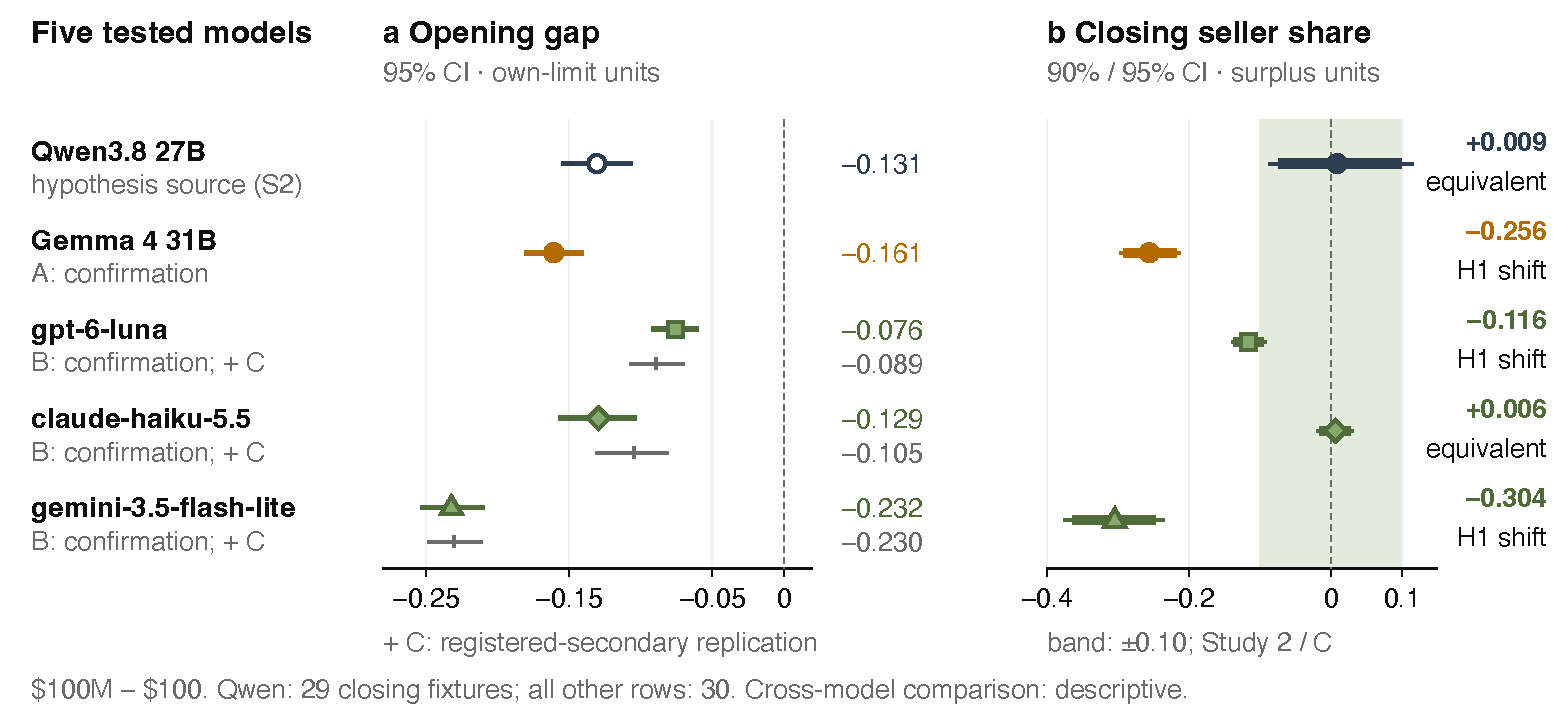
\includegraphics[width=0.92\textwidth]{../manuscript/figures/main_models.pdf}
  \caption{Shared opening modesty, model-dependent closing splits (discovery phase). (a) Mean opening-gap change with 95\% CIs: Qwen is the descriptive hypothesis source; Gemma A and API B estimates are confirmatory; offset API C estimates are registered-secondary replications. (b) Primary closing shifts from Study 2 and C, using all agreements: thick bars 90\%, thin bars 95\%, band $\pm 0.10$.}
  \label{fig:app-models}
\end{figure}

In Addendum C, prospective midpoint accounting (Figure~\ref{fig:app-midpoint}) confirmed tracking (HM2) on all three API models (Spearman $\rho = 0.774, 0.605, 0.847$; Holm $p = 0.00015$ each) and calibration (HM1, $\pm 0.05$) on Luna ($e = -0.009$, 90\% CI [$-0.025, +0.009$]), while Haiku ($+0.025$ [$-0.008, +0.060$]) and Gemini ($-0.043$ [$-0.073, -0.014$]) did not establish $\pm 0.05$ equivalence. Directly clamping openings in Study 3 (Section~\ref{sec:res-clamp}) later tested the causal channel prospectively.

\begin{figure}[t]
  \centering
  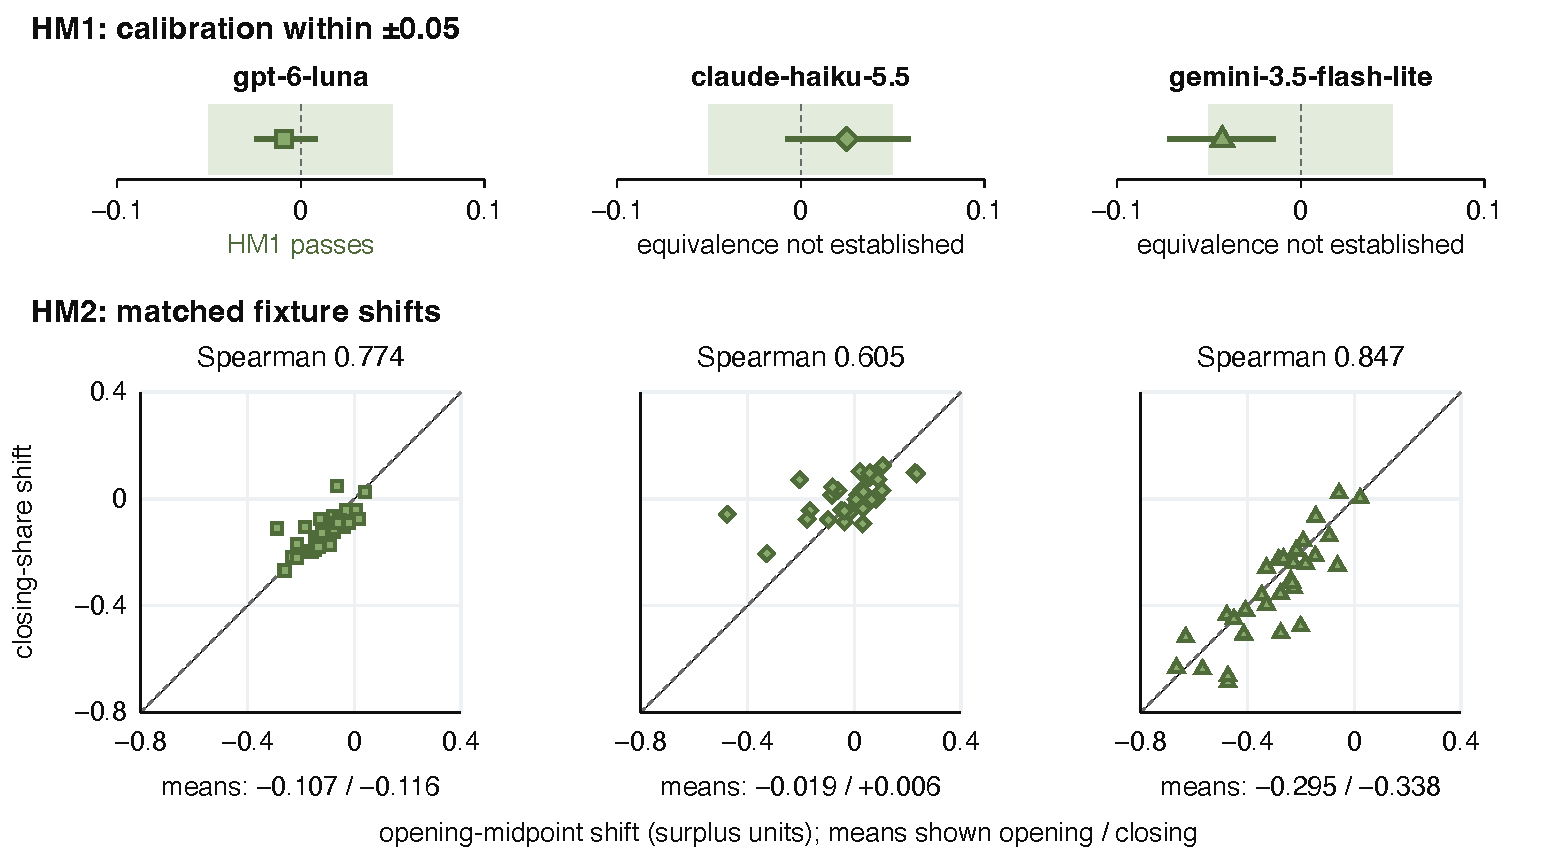
\includegraphics[width=0.90\textwidth]{../manuscript/figures/main_midpoint.pdf}
  \caption{Prospective midpoint accounting in Addendum C. Top: mean closing-minus-midpoint shift with 90\% CI and the $\pm 0.05$ HM1 margin. Bottom: matched fixture shifts (30 per model), with equality shown dashed.}
  \label{fig:app-midpoint}
\end{figure}

\subsection{Exploratory behavioural probes and midpoint decomposition (D.10)}
\label{app:d10}

All analyses in this subsection are exploratory. Figures~\ref{fig:app-probes}, \ref{fig:app-midpoint-open}, \ref{fig:app-map}, and~\ref{fig:app-digits} display the probe results summarised in Section~\ref{sec:res-controls}.

\begin{itemize}
  \item \textbf{Redesigned-game probe (X17, 600 games).} The Study 2 bridge on L01--L30 replicated Gemma's shift ($-0.253$, 95\% CI [$-0.296, -0.209$], 29/30 negative). Redesigned self-play with off-centre ranges, business notation, and cents gave $+0.027$ [$-0.036, +0.088$] after excluding comma-truncated prices (68 slipped games at $\times 10^6$), while both opening gaps still fell (16.5 points for sellers, 9.2 for buyers). Against a scale-invariant scripted bot, Gemma's seller-share change was $-0.258$ [$-0.318, -0.199$] (27/28 fixtures negative).
  \item \textbf{Geometry and notation probes (X18, X22, 2{,}160 games per model).} Crossing Study 2's round-centred zone, a narrow off-centre zone, and a wide zone with raw and business notation gave raw Gemma self-play shifts of $-0.21$, $-0.20$, and $-0.06$ (attenuated by 0.03--0.09 under business notation). Qwen's raw narrow-zone shift was $-0.12$ [$-0.21, -0.03$].
  \item \textbf{Cross-play (X19, 960 games).} Gemma selling to Qwen shifted by $-0.113$, whereas Qwen selling to Gemma shifted by $-0.042$ (non-significant).
  \item \textbf{Instruction probes (X20--X21, 2{,}160 games per model).} Crossing no addition, tough, cooperative, and scale-neutral instructions retained opening shrinkage in every style: 6--13 points for Qwen; 38--47\% of the seller gap and 18--24\% of the buyer gap for Gemma. The exact scale-neutral text was: \emph{``The size of the numbers does not change what good negotiating looks like. Negotiate exactly as you would if every amount were a thousand times smaller or a thousand times larger.''}
  \item \textbf{Information probes (X23--X24, 1{,}560 games per model).} Privately supplying the other side's range pinned Gemma's openings (120/120 buyers at \$75/\$75M; 118/120 sellers at \$120/\$120M) and removed its bot loss (moving from $-0.14$ to $+0.01$; Qwen likewise removed its bot loss). When both sides were told the other's range (X26--X27), Gemma's self-play split still fell by $-0.083 = -0.019 - 0.064$ ($\approx 77\%$ in concessions), whereas Qwen's concession term was $+0.029$ (Figure~\ref{fig:app-midpoint-open}).
  \item \textbf{Digits and cents probes (X15--X16, 1{,}920 + 1{,}680 first moves on Gemma, Y01--Y30).} Keeping digits fixed and changing the unit to millions gave 61\% of the full shift ($-8.9$ of $-14.5$ points; 30/30 negative); changing the digit string at fixed stakes supplied the remaining $-5.6$ points (28/30 negative). Plain small-dollar wording produced 99\% round-ten seller openings (vs.\ 35--57\% under other initial wordings); ``81.00 dollars'' retained 97\% round tens, and adding ``\$'' shifted the both-role gap by only 2--3 points (Figure~\ref{fig:app-digits}).
\end{itemize}

\begin{figure}[t]
  \centering
  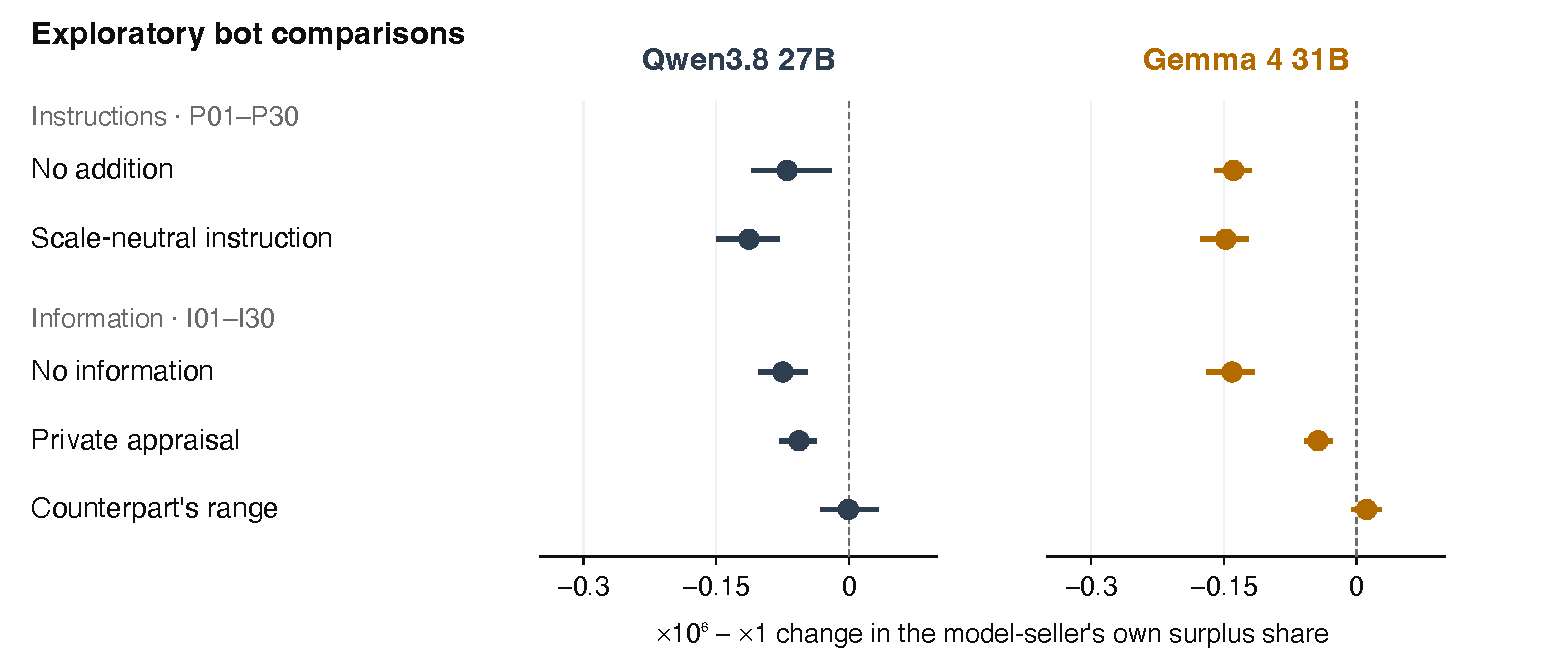
\includegraphics[width=0.90\textwidth]{../manuscript/figures/main_probes.pdf}
  \caption{Instruction and information against a scale-invariant counterpart (exploratory). Change in the model-seller's own surplus share at $\times 10^6$, with 95\% fixture-bootstrap CIs. The scale-neutral instruction retains the loss; knowledge of the counterpart's range removes it in these runs.}
  \label{fig:app-probes}
\end{figure}

\begin{figure}[t]
  \centering
  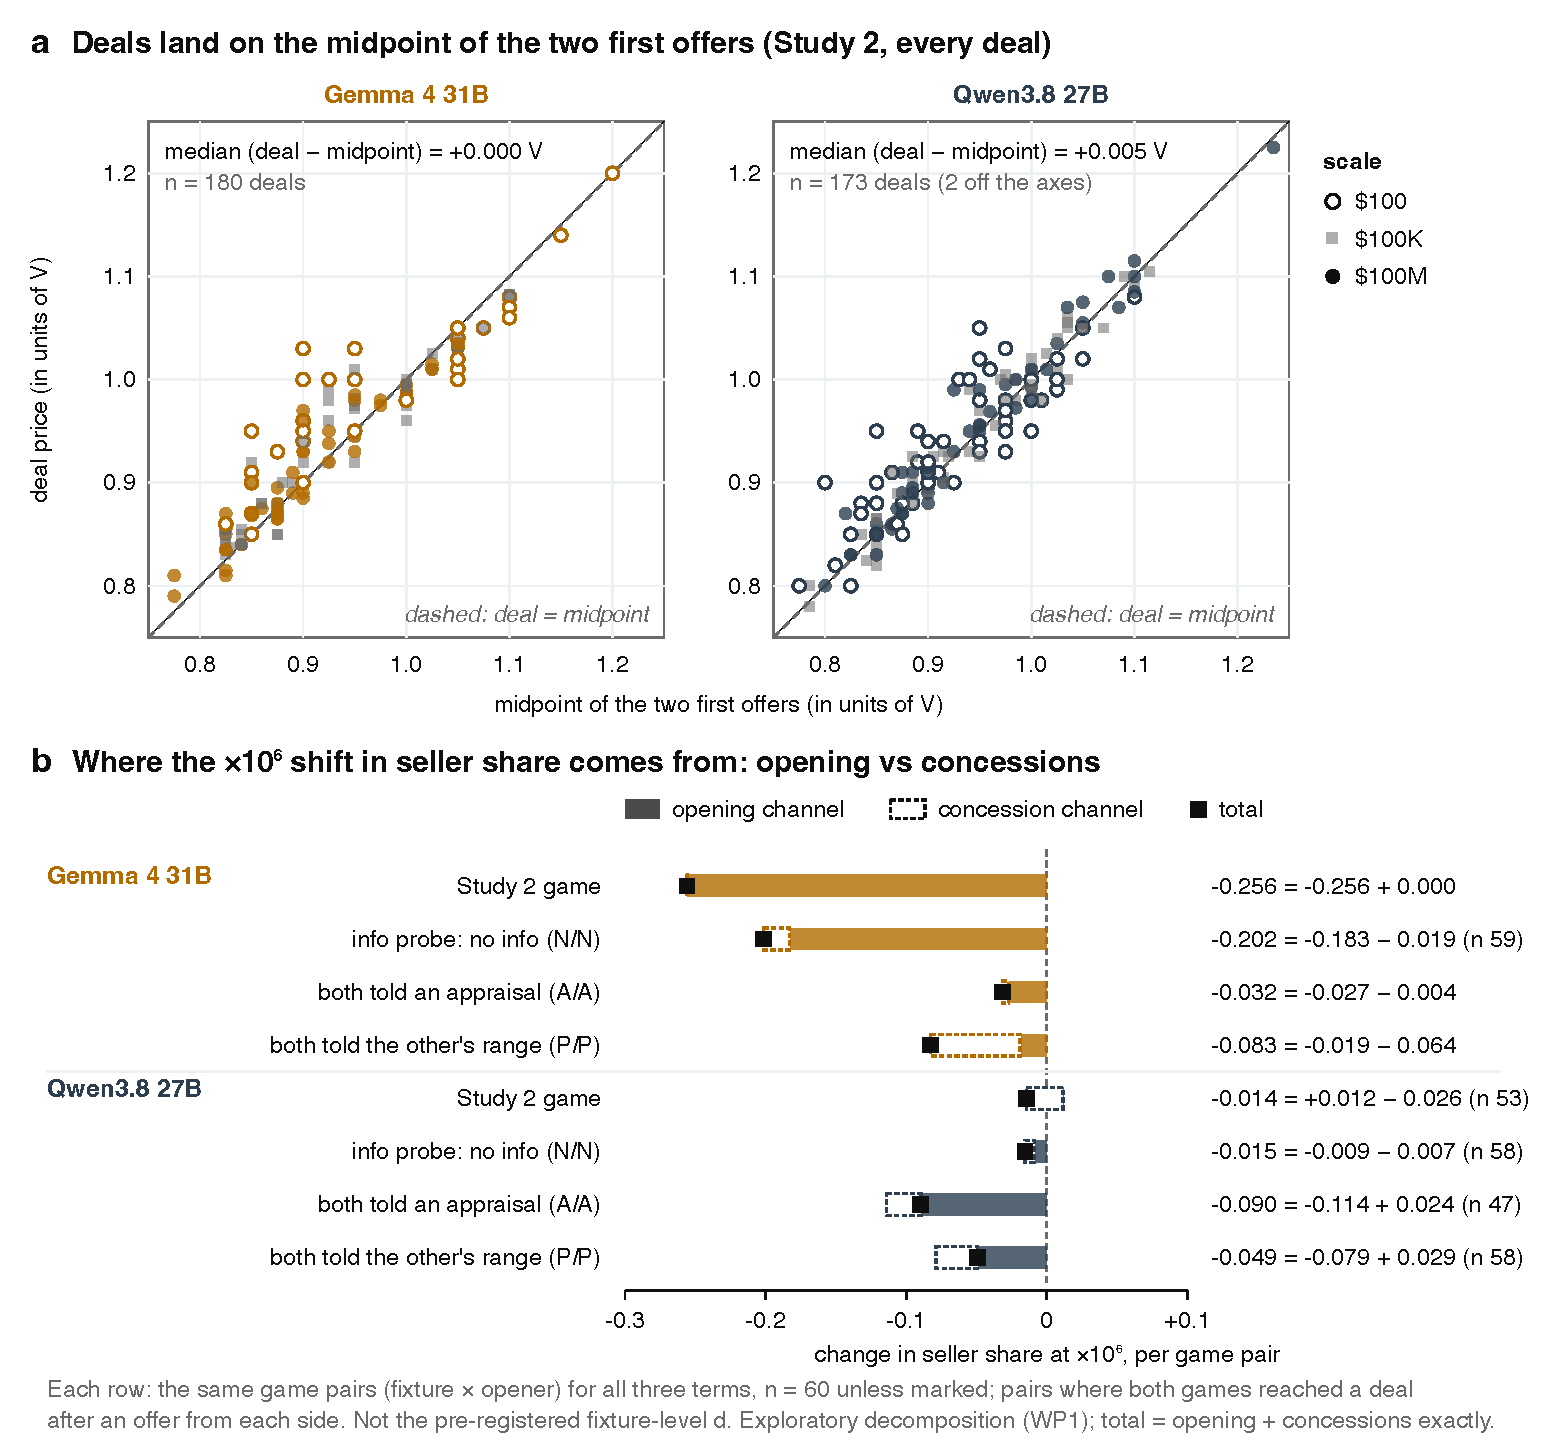
\includegraphics[width=0.90\textwidth]{../manuscript/figures/fig4_midpoint.pdf}
  \caption{Exploratory open-model midpoint and concession accounting. Upper panels compare deals with the in-game first-offer midpoint; lower panel decomposes changes on identical eligible game pairs.}
  \label{fig:app-midpoint-open}
\end{figure}

\begin{figure}[t]
  \centering
  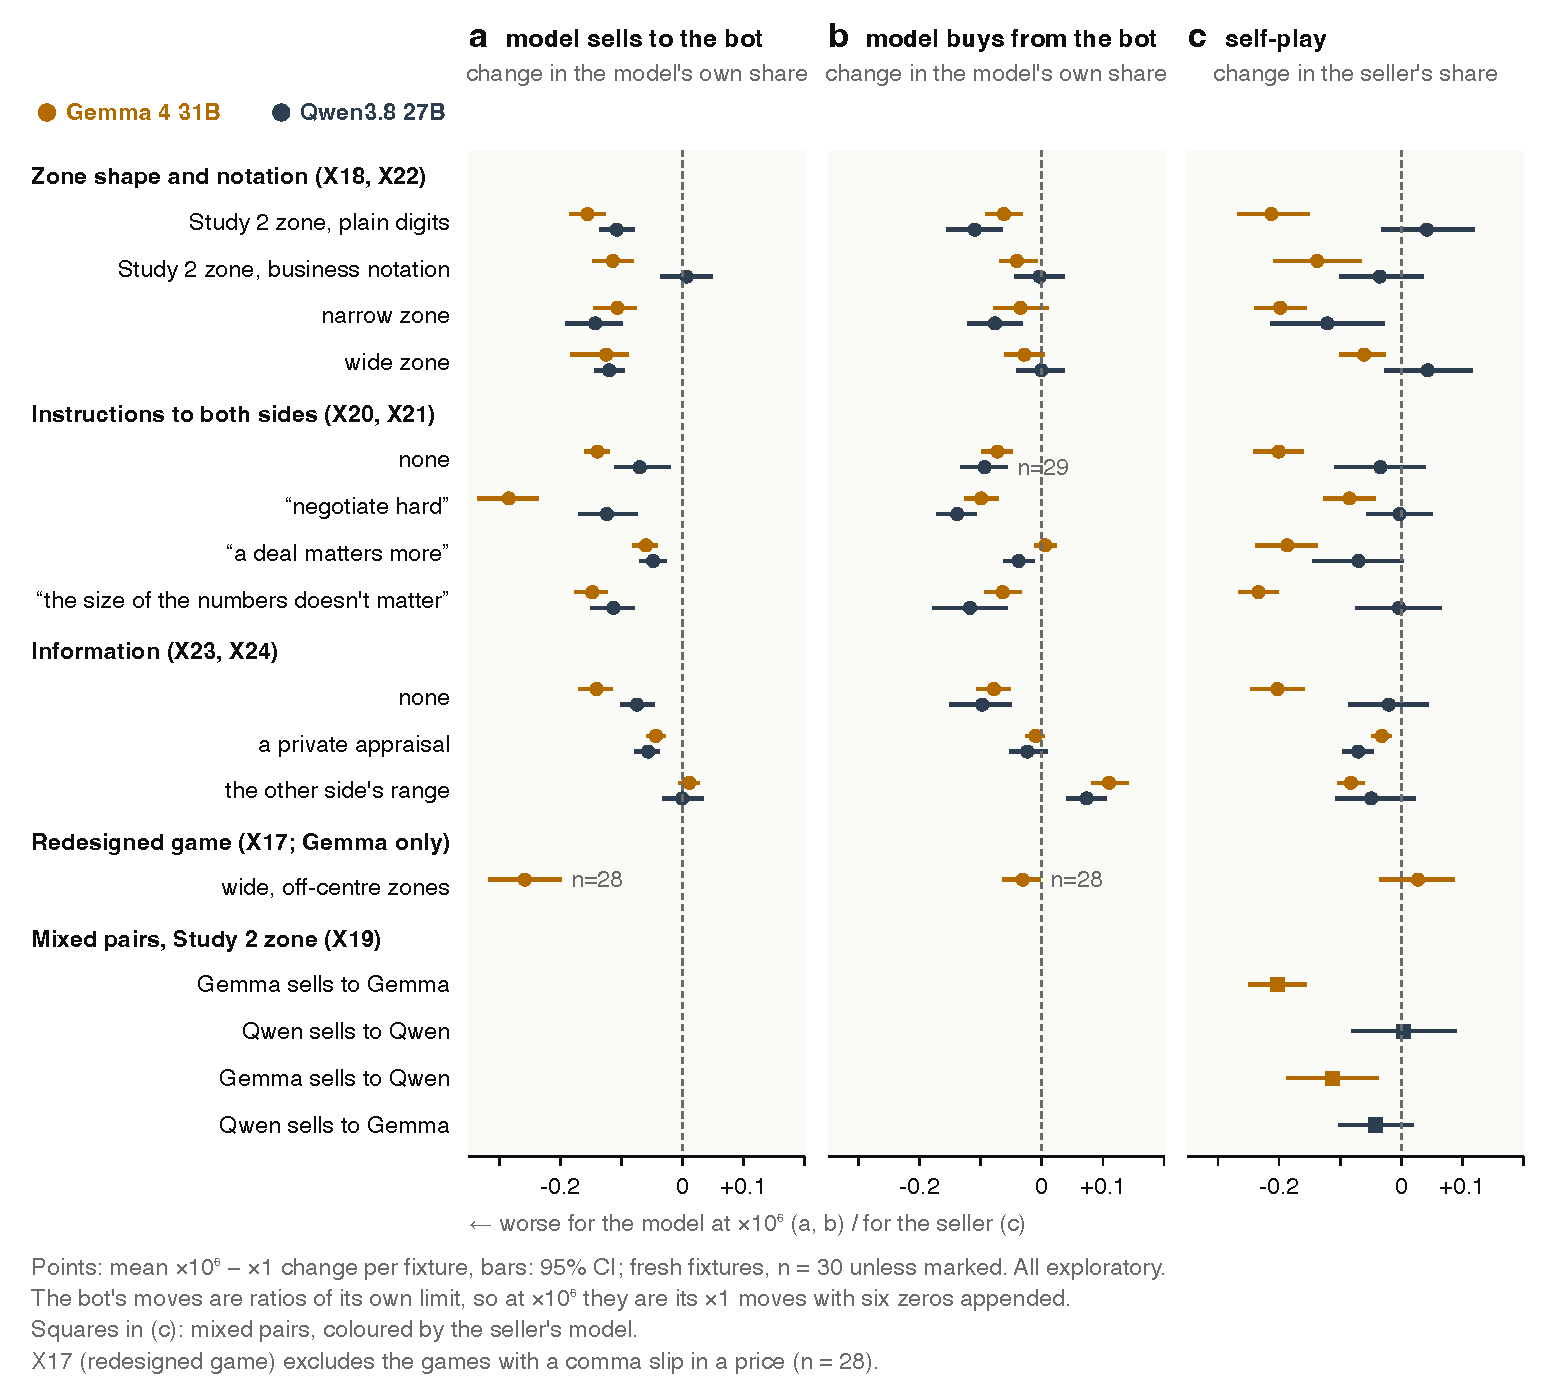
\includegraphics[width=0.92\textwidth]{../manuscript/figures/fig5_map.pdf}
  \caption{Full exploratory behavioural comparison across probe families (95\% CIs). Bot columns use the model's own share, self-play the seller's share.}
  \label{fig:app-map}
\end{figure}

\begin{figure}[t]
  \centering
  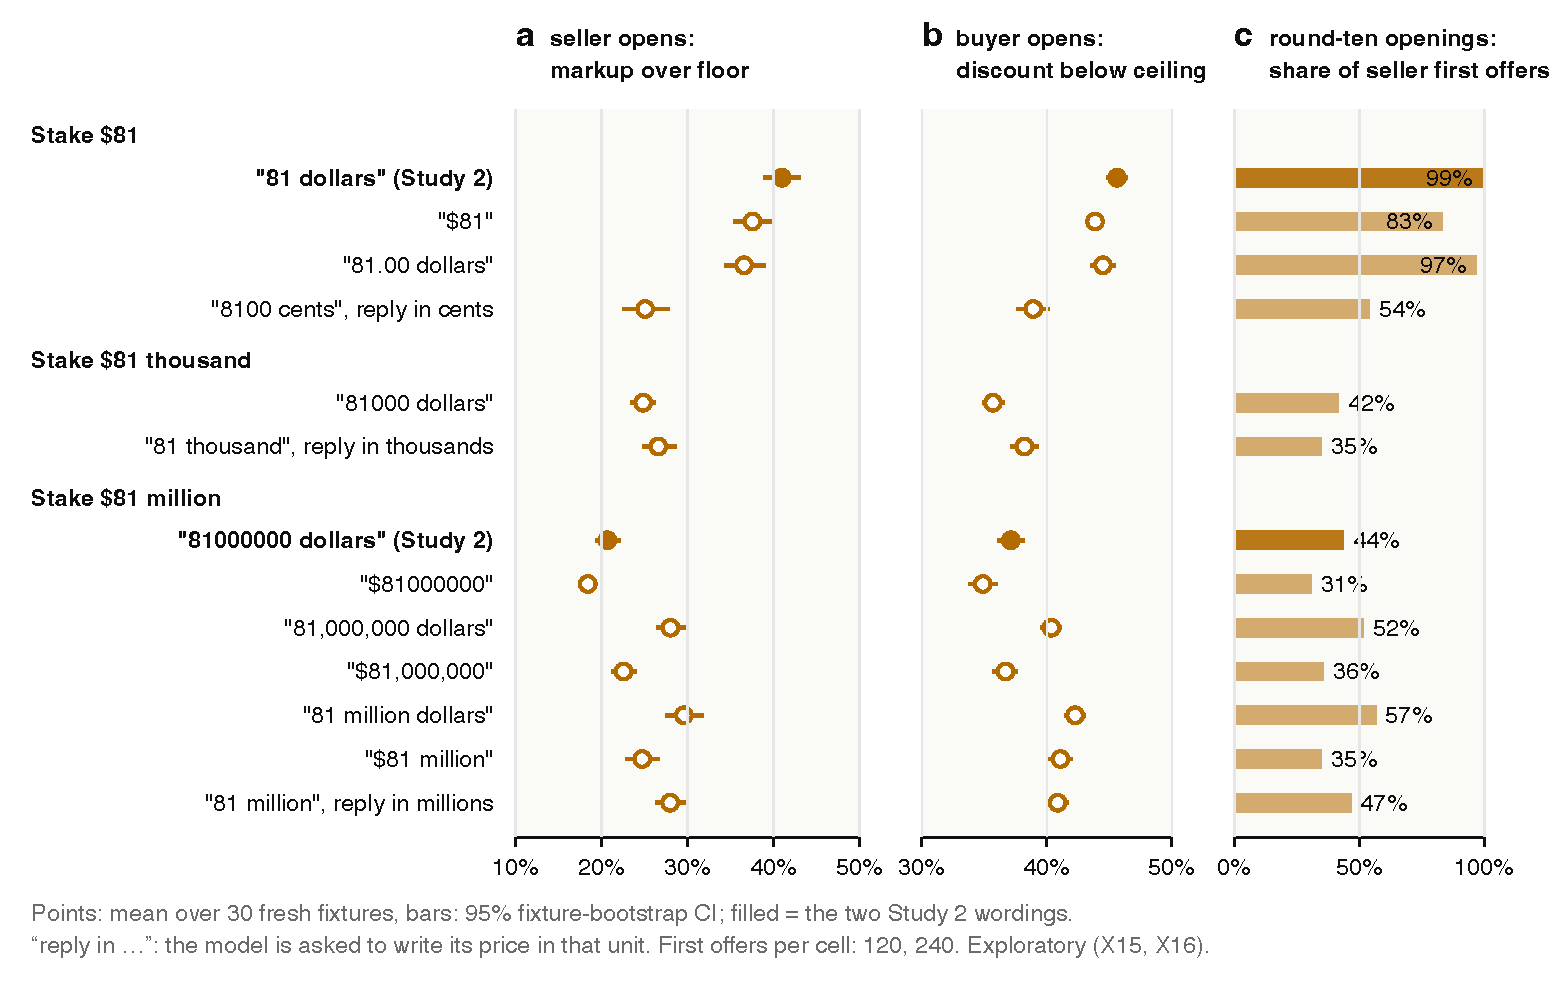
\includegraphics[width=0.92\textwidth]{../manuscript/figures/fig6_digits.pdf}
  \caption{The full 13-wording comparison in Gemma (X15--X16, exploratory). Seller markup, buyer discount, and round-ten seller openings on fresh fixtures (95\% CIs).}
  \label{fig:app-digits}
\end{figure}

\subsection{Discovery-phase mechanistic programme (D.11)}

The discovery-phase mechanistic programme (X51--X64) instrumented Gemma 4 31B in bf16 on 30 fresh fixtures (Y01--Y30). Key findings that motivated E5 and E6: (i) magnitude is linearly decodable from limit digits early ($R^2 = 0.98$--$0.99$ from layer 5; \citealp{belinkov2021probing}), while behavioural patching becomes decisive at layers 41--47 (restoring 82\% [73, 90] of the gap); (ii) prompt-only steering at layer 44 failed ($\le 17\%$), whereas including the reply's 11 opening tokens enabled bidirectional steering of real openings (74--95\% at unit strength across layers 42, 44, and 48; 109--176\% at double strength; non-money control $\le 14\%$; Figure~\ref{fig:app-mech}); (iii) six operationalised concept directions (count, money, million, digits, stakes, modesty) held up to a third of the scale direction's squared norm at layers 41--42, yet their projection moved real openings only 0--6\% while the orthogonal remainder moved 84--86\% (Figure~\ref{fig:app-concepts}; \citealp{singh2024tokenization, elshangiti2024geometry, tan2024steeringreliability, lekeas2026nashcircuit}).

\begin{figure}[t]
  \centering
  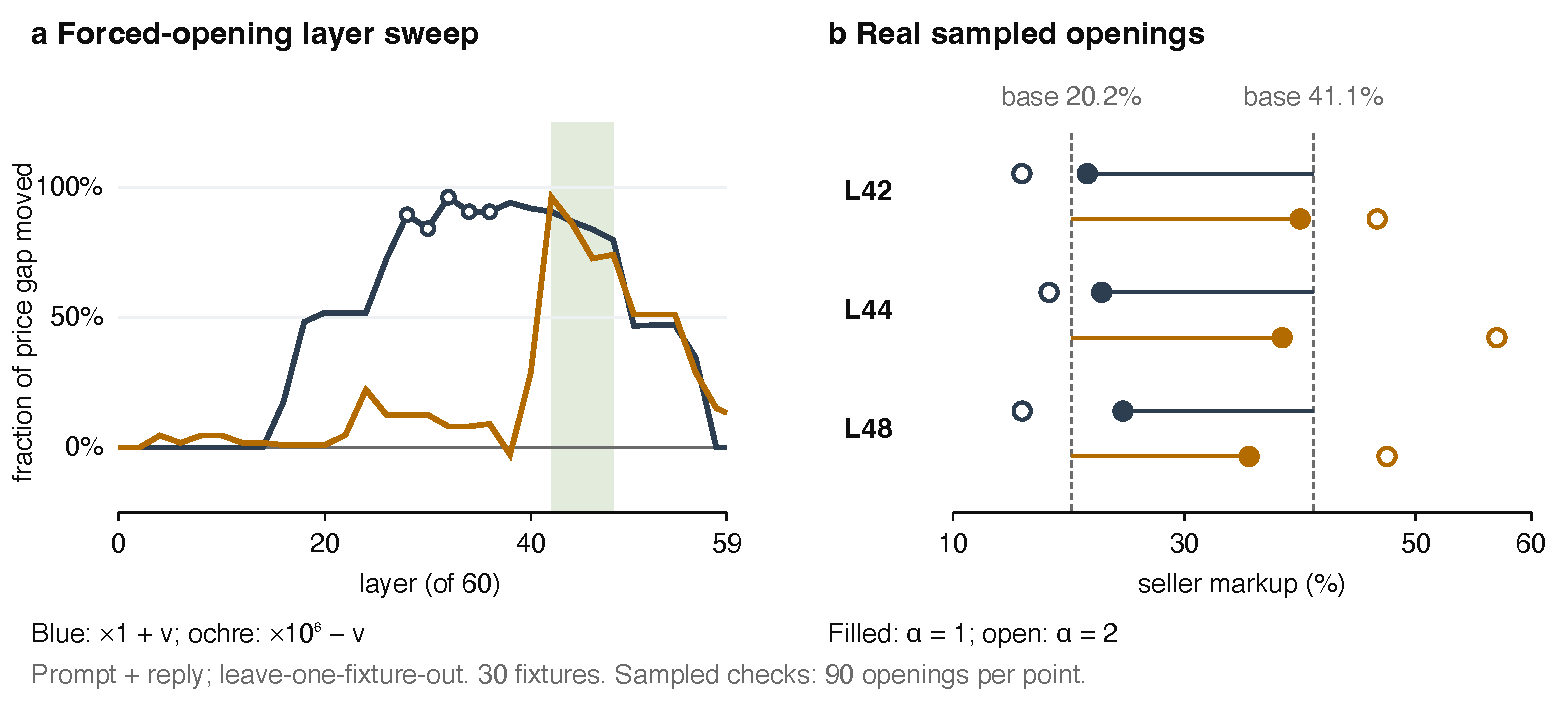
\includegraphics[width=0.92\textwidth]{../manuscript/figures/main_mechanism.pdf}
  \caption{Late bidirectional steering site in Gemma (discovery phase, exploratory). (a) Forced-opening layer sweep; (b) real sampled openings at layers 42, 44, and 48 (all 1{,}080 steered replies format-valid).}
  \label{fig:app-mech}
\end{figure}

\begin{figure}[t]
  \centering
  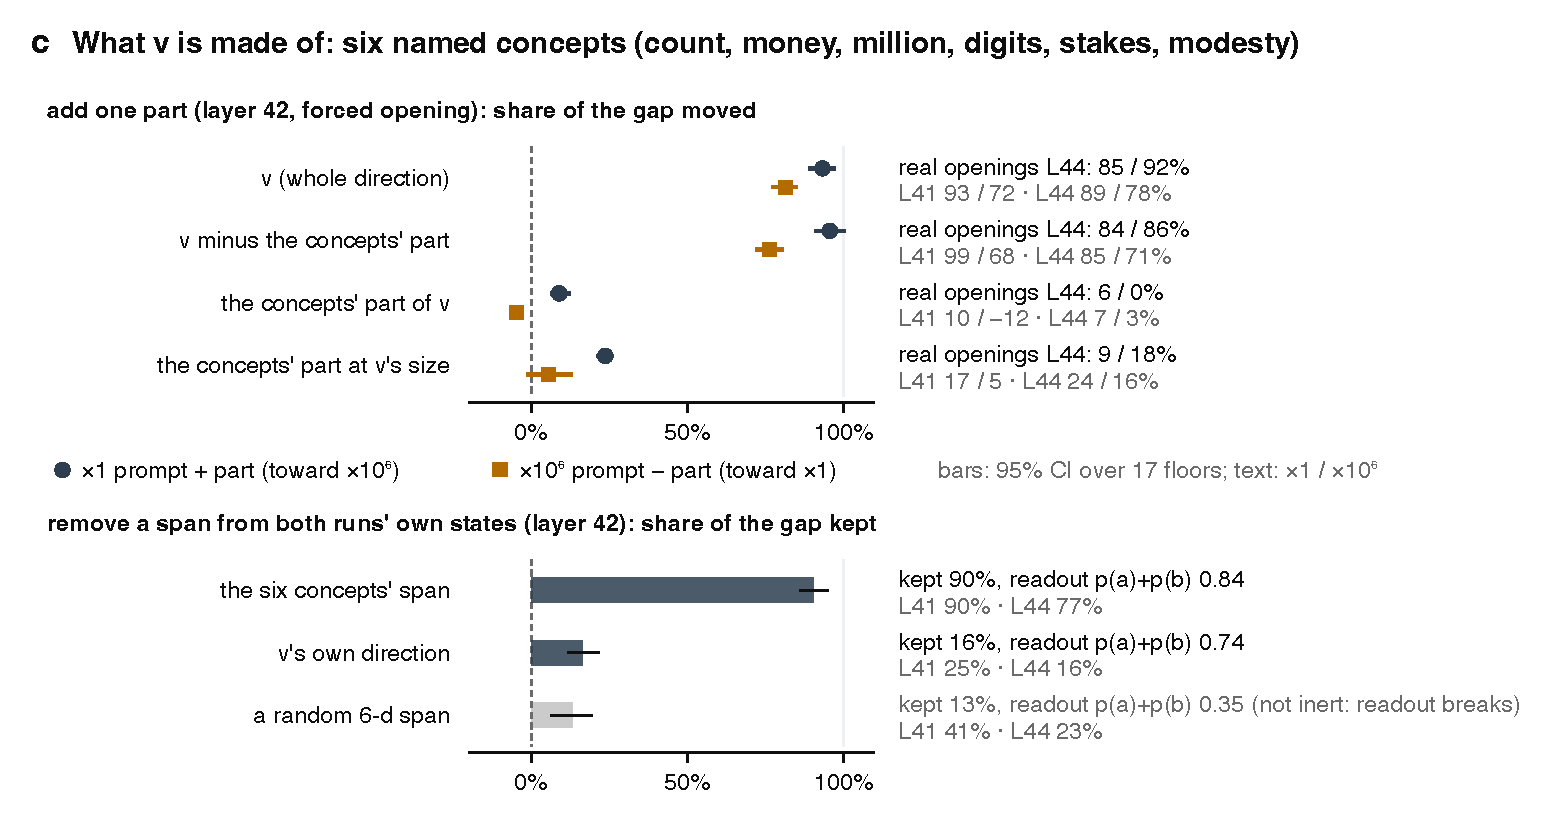
\includegraphics[width=0.92\textwidth]{../manuscript/figures/app_concepts_detail.pdf}
  \caption{Concept projection, orthogonal remainder, and ablation controls on 17 distinct seller floors (X63--X64, exploratory, 95\% CIs).}
  \label{fig:app-concepts}
\end{figure}

\section{E5 methods and full results}
\label{app:e5}

Run \texttt{interp-e5-gemma-4-31b-it-20261015T232511Z} (39 minutes of GPU time, \$1.62 estimated); predictions committed in \texttt{config/interp/e5\_predictions.md} (SHA-256 \texttt{ba05f2c2\ldots}, commit \texttt{0d8b715}) before the run.

\paragraph{Design and readout.} One Study 3 fixture per distinct limit among G01--G40 (19 seller floors: 7 discovery floors G01--G07 and 12 held-out floors; 18 buyer ceilings, 17 usable). Forced openings fix the reply prefix through \texttt{\{"action": "OFFER", "price":} and read the log-odds at the first differing digit between the limit's two A0 greedy prices. Sellers' A0 scale gap is $G_N = 18.4$ nats and A1 gap is $3.0$ nats (17\%; E5-1); buyers' are $7.1$ and $0.7$ nats (10\%). Probability mass on the two deciding tokens is 0.83--0.87 in \$100M runs except buyers' A1 run (\eFiveBuyerProbMass{}).

\begin{table}[t]
  \centering
  \caption{E5 pre-committed exploratory predictions and outcomes.}
  \label{tab:e5-preds}
  \small
  \begin{tabular}{@{}lp{0.50\textwidth}p{0.36\textwidth}@{}}
    \toprule
    ID & Prediction & Outcome \\
    \midrule
    E5-1 & Under A1, sellers' forced opening keeps 5--50\% of the A0 scale gap & Hit: \eFiveGapShare{} \\
    E5-2 & Adding appraisal moves $\le 15\%$ at every layer $\le 39$ and $\ge 50\%$ at L41 or L42 & Hit by signed rule ($+0.5\%$; 83\%); moves 13--35\% wrong way at L30--40 \\
    E5-3 & At L44, reply opening tokens move more than prompt final segment & Hit: \eFiveReplyShare{} vs.\ \eFivePromptShare{} \\
    E5-4 & A0 scale direction moves A1 openings $< 0.5\times$ as much as A0 openings & Hit: \eFiveSteerAoneLow{}--\eFiveSteerAoneHigh{} vs.\ \eFiveSteerAzeroLow{}--\eFiveSteerAzeroHigh{} \\
    E5-5 & $\ge 2$ of top 8 heads shared with scale/range heads; 8 carry $\ge 50\%$ held-out & Overlap hit (\eFiveHeadOverlap{} of 8); reg.\ ratio (\eFiveHeldOutRatio{}) uninterpretable; post-hoc direct share \eFiveHeldOutOwnGapPct{} (12/12 floors) \\
    E5-6 & Buyers show the same onset as E5-2 & Miss: buyers enter gradually from L30 \\
    \bottomrule
  \end{tabular}
\end{table}

% Auto-generated from E5 summary.json
\begin{table}[t]
\centering
\caption{E5 behavioural gate comparing four sampled \texttt{transformers} openings per prompt against Study 3's vLLM openings on the same prompts. Both roles passed the pre-committed gate (all cells and shifts within 3 points; $\ge 95\%$ valid).}
\label{tab:e5-gate}
\footnotesize
\setlength{\tabcolsep}{4pt}
\begin{tabular}{@{}llrrrrrr@{}}
\toprule
Role & Cell & Valid / $n$ & Off-scale & Gap (\texttt{transformers}) & Gap (vLLM) & Prompts & Per-prompt $r$ \\
\midrule
Sellers & A0, \$100 & 76 / 76 & 0 & 44.6\% & 44.5\% & 19 & 0.97 \\
Sellers & A0, \$100M & 76 / 76 & 0 & 22.1\% & 22.5\% & 19 & 0.97 \\
Sellers & A1, \$100 & 76 / 76 & 0 & 37.6\% & 36.7\% & 19 & 1.00 \\
Sellers & A1, \$100M & 76 / 76 & 0 & 34.5\% & 34.1\% & 19 & 0.99 \\
Buyers & A0, \$100 & 72 / 72 & 17 & 44.8\% & 46.0\% & 15 & 0.38 \\
Buyers & A0, \$100M & 72 / 72 & 0 & 35.7\% & 35.9\% & 18 & 0.81 \\
Buyers & A1, \$100 & 72 / 72 & 0 & 31.5\% & 31.6\% & 18 & 0.94 \\
Buyers & A1, \$100M & 72 / 72 & 0 & 24.6\% & 25.1\% & 18 & 0.99 \\
\bottomrule
\end{tabular}
\end{table}

% Auto-generated from E5 summary.json
\begin{table}[t]
\centering
\caption{E5 appraisal swap by layer and token segment at \$100M (share of forced-opening log-odds distance between A0 and A1; sellers 19 floors, buyers 17 ceilings).}
\label{tab:e5-swap}
\small
\begin{tabular}{@{}lrrrr@{}}
\toprule
Layer / segment & Sellers, adding & Sellers, removing & Buyers, adding & Buyers, removing \\
\midrule
0 & $-$2\% & 0\% & 0\% & $-$1\% \\
10 & $-$1\% & $+$1\% & $-$1\% & 0\% \\
20 & $-$1\% & $+$1\% & $-$2\% & $+$1\% \\
24 & $-$3\% & $-$3\% & $-$11\% & $+$4\% \\
26 & $-$8\% & $-$6\% & $-$3\% & $+$7\% \\
28 & $-$13\% & $-$8\% & $+$5\% & $+$7\% \\
30 & $-$13\% & $-$15\% & $+$18\% & $+$13\% \\
32 & $-$20\% & $-$26\% & $+$30\% & $+$19\% \\
34 & $-$26\% & $-$45\% & $+$30\% & $+$25\% \\
36 & $-$30\% & $-$59\% & $+$38\% & $+$42\% \\
37 & $-$36\% & $-$58\% & $+$37\% & $+$43\% \\
38 & $-$35\% & $-$61\% & $+$40\% & $+$49\% \\
39 & $-$27\% & $-$40\% & $+$40\% & $+$65\% \\
40 & $-$23\% & $-$27\% & $+$37\% & $+$63\% \\
41 & $+$75\% & $+$78\% & $+$89\% & $+$79\% \\
42 & $+$83\% & $+$92\% & $+$89\% & $+$82\% \\
43 & $+$87\% & $+$90\% & $+$89\% & $+$82\% \\
44 & $+$88\% & $+$89\% & $+$87\% & $+$82\% \\
46 & $+$89\% & $+$85\% & $+$85\% & $+$82\% \\
48 & $+$99\% & $+$102\% & $+$90\% & $+$84\% \\
52 & $+$104\% & $+$113\% & $+$98\% & $+$95\% \\
56 & $+$105\% & $+$108\% & $+$98\% & $+$98\% \\
59 & $+$111\% & $+$113\% & $+$101\% & $+$103\% \\
\midrule
41, S tokens only & $+$18\% & $+$24\% & $+$21\% & $+$3\% \\
44, S tokens only & $+$22\% & $+$27\% & $+$16\% & $+$3\% \\
48, S tokens only & $+$15\% & $+$23\% & $+$11\% & $+$5\% \\
52, S tokens only & $+$8\% & $+$19\% & $+$11\% & $+$8\% \\
41, reply tokens only & $+$50\% & $+$49\% & $+$77\% & $+$62\% \\
44, reply tokens only & $+$57\% & $+$58\% & $+$78\% & $+$68\% \\
48, reply tokens only & $+$72\% & $+$82\% & $+$80\% & $+$73\% \\
52, reply tokens only & $+$81\% & $+$103\% & $+$88\% & $+$85\% \\
\bottomrule
\end{tabular}
\end{table}

% Auto-generated from E5 summary.json
\begin{table}[t]
\centering
\caption{E5 top eight appraisal-swap heads (layers 38--44, 224 heads) ranked on the 7 discovery floors, and overlap with the discovery-phase scale (X57) and range (X61) head sets (6 of 8 shared; chance $\approx 0.46$).}
\label{tab:e5-heads}
\small
\begin{tabular}{@{}lrcc@{}}
\toprule
Head (layer.head) & Score (discovery) & In scale set (X57) & In range set (X61) \\
\midrule
41.11 & 0.540 & yes & yes \\
41.26 & 0.175 & --- & --- \\
41.8 & 0.130 & --- & yes \\
41.29 & 0.123 & yes & yes \\
43.5 & 0.091 & yes & yes \\
42.9 & 0.077 & yes & --- \\
40.13 & 0.067 & --- & --- \\
39.2 & 0.065 & --- & yes \\
\bottomrule
\end{tabular}
\end{table}

% Auto-generated from E5 held-out circuit table
\begin{table}[t]
\centering
\caption{E5 held-out floors (12): patching the eight appraisal heads' A1 outputs into the A0 \$100M run. Negative moves are toward the \$100 price (12/12 floors). The pre-committed E5-5 ratio ($1.88$) divides by the sign-changing A1 $-$ A0 denominator ($-26.0$ to $+7.1$ nats) and is not a bounded share; the direct share of each floor's own A0 scale gap (mean 67\%, vs.\ 0\% for 8 random heads) is the well-conditioned readout reported in Section~\ref{sec:interp}.}
\label{tab:e5-circuit}
\footnotesize
\setlength{\tabcolsep}{4pt}
\begin{tabular}{@{}lrrrrrr@{}}
\toprule
Floor & Floor (\$100) & 8-head move & Own A0 gap & Share of gap & Reg.\ denom. & 8 rand.\ heads \\
\midrule
G08 & \$93 & $-$5.00 & $+$13.12 & 38\% & $+$5.12 & $+$0.25 \\
G12 & \$78 & $-$17.62 & $+$19.69 & 90\% & $-$22.50 & $-$0.25 \\
G13 & \$80 & $-$13.75 & $+$27.44 & 50\% & $+$0.19 & 0.00 \\
G14 & \$91 & $-$6.12 & $+$12.00 & 51\% & $+$4.25 & 0.00 \\
G15 & \$77 & $-$19.38 & $+$23.06 & 84\% & $-$26.00 & 0.00 \\
G17 & \$86 & $-$15.62 & $+$19.62 & 80\% & $-$11.00 & 0.00 \\
G18 & \$88 & $-$7.50 & $+$13.50 & 56\% & $+$1.25 & $-$0.25 \\
G20 & \$83 & $-$14.00 & $+$16.31 & 86\% & $-$19.25 & $-$0.25 \\
G21 & \$90 & $-$15.75 & $+$22.88 & 69\% & $+$5.38 & $-$0.12 \\
G23 & \$85 & $-$9.38 & $+$13.62 & 69\% & $-$4.00 & $-$0.12 \\
G27 & \$79 & $-$15.88 & $+$18.44 & 86\% & $-$20.75 & 0.00 \\
G37 & \$95 & $-$10.75 & $+$24.62 & 44\% & $+$7.12 & 0.00 \\
\midrule
\textbf{Mean} &  & \textbf{$-$12.56} & \textbf{$+$18.69} & \textbf{67\%} & \textbf{$-$6.68} & \textbf{$-$0.06} \\
\bottomrule
\end{tabular}
\end{table}

\FloatBarrier

\section{E6 methods and full results}
\label{app:e6}

Run \texttt{interp-e6-gemma-4-31b-it-20261016T013146Z} (14 minutes of GPU time, \$0.58 estimated); predictions committed in \texttt{config/interp/e6\_predictions.md} (SHA-256 \texttt{72274e9c\ldots}, commit \texttt{c892fff}) before the run. Table~\ref{tab:e6-preds} scores all ten pre-committed predictions.

\begin{table}[t]
  \centering
  \caption{E6 pre-committed exploratory predictions and outcomes.}
  \label{tab:e6-preds}
  \small
  \begin{tabular}{@{}lp{0.52\textwidth}p{0.34\textwidth}@{}}
    \toprule
    ID & Prediction & Outcome \\
    \midrule
    E6-1 & Negotiation direction (L42, $\alpha = +2$) moves \$100 openings $\ge 40\%$; random $\le 10\%$ & Hit: \eSixNegMove{}; random \eSixNegRand{} \\
    E6-2 & Digits direction reads words and short notation at $r \ge 0.8$ in L10--40 & Hit: $r = 0.97$ (lower of two at best layer) \\
    E6-3 & Transfer to words at L0--2 is $\ge 0.2$ below peak & Hit: $0.61$ vs.\ $0.98$ \\
    E6-4 & Money direction reads people counts at $r \ge 0.8$ & Trivial (L0): $0.94$ already at L0 (shared digits) \\
    E6-5 & Risky choices are safer at \$100M by $\ge 0.5$ nats & Hit: \eSixRiskNatGap{} nats \\
    E6-6 & Direction moves risky choices $\ge 25\%$ of gap and $> 3\times$ controls & Miss: \eSixRiskMove{}; control \eSixRiskCtrl{} \\
    E6-7 & Same for percentage answers & Miss: \eSixPctMove{}; control \eSixPctCtrl{} \\
    E6-8 & Comparisons and sums are intact under the direction & Hit \\
    E6-9 & Fermi estimates move $\le 0.15$ $\log_{10}$ at $\alpha = \pm 2$ & Miss: $+$\eSixFermiPlus{} and $-$\eSixFermiMinus{} (control $+0.97$) \\
    E6-10 & $|\cos(\text{digits direction}, \text{negotiation direction})| \le 0.2$ at L42 & Miss: \eSixCos{} \\
    \bottomrule
  \end{tabular}
\end{table}

\paragraph{Part A (number).} 360 sentences (mantissas 12, 23, 37, 45, 58, 64, 73, 81, 96 $\times$ $10^0$--$10^7$) in five notations (digits, words, short, commas, people count), read at the final period. A magnitude direction is the per-layer covariance of the residual state with $\log_{10}$ amount within one notation; transfer is Pearson $r$ on other notations. The MLP census inspects the down-projection input at layers 4, 10, 20, 30, and 41. Three scoring artefacts: (1) E6-4 transfers at $r = 0.94$ already at layer 0 due to shared digit strings; (2) the pre-committed exponent-tuning count ($z \ge 3$ across 8 exponents) is mathematically unreachable ($\max z = 7/\sqrt{8} \approx 2.47$) and omitted; (3) the random Gaussian vector at $\alpha = \pm 2$ leaves mean probability $0.006$ on valid options in short risk/comparison prompts and breaks parsing on 15/15 percentage prompts in two cells, so its shares there are uninterpretable.

\paragraph{Part B (stakes).} $v_R$ is the mean of the reply-token rows of E5's seller scale difference at layers 42 and 44 ($|v_R| = 30.4$ at layer 42; reply coherence $0.79$); $v_S$ uses the prompt's S tokens ($\cos = 0.85$ with $v_R$); $u$ is the non-money contrast ($\cos = 0.35$); $\text{rand}$ is a seeded Gaussian vector scaled to $|v_R|$. Risky choices by expected-value ratio (safe-option log-odds, mean of 10 prompts): equal EV, $+18.5$ at \$100 and $+20.2$ at \$100M; gamble worth $1.2\times$, $-16.9$ and $-2.6$; gamble worth $1.5\times$, $-11.6$ and $+2.5$. Steered shares at layer 42, $\alpha = +2$, on \$100 prompts: negotiation $v_R$ 86\%, $v_S$ 73\%, $u$ 8\%, rand 8\%; risk $v_R$ 4.9\%, $u$ 1.5\%; percentages $v_R$ $-4.4\%$, $u$ $-2.2\%$. Fermi shifts ($\log_{10}$): $v_R$ $+0.46$ ($\alpha = +1$), $+1.15$ ($+2$), $-0.29$ ($-1$), $-0.50$ ($-2$); $u$ $+0.97$; median item moves $0.04$ at $v_R$ $\alpha = +2$.

% Auto-generated from derived/addendum_d/addendum_d_all.json
\begin{table}[t]
\centering
\caption{E6b layer-covariance-matched, format-orthogonalized random control (\texttt{rand\_cov}, L42, $|\text{rand\_cov}| = |v_R| = 30.39$, $\cos(v_R, \text{rand\_cov}) = 0.000$) vs.\ isotropic \texttt{rand}, non-money control $u$, and negotiation direction $v_R$ at $\alpha = +2$ on \$100 prompts (Gemma 4 31B). Unlike isotropic \texttt{rand} (which collapses valid-option mass to $0.000$), \texttt{rand\_cov} preserves $1.00$ valid-option mass and $100\%$ parse rate while remaining inert on risky choices ($-3.5\%$; $-0.2\%$ at $\alpha=+1$) and percentages ($+2.9\%$).}
\label{tab:e6b}
\footnotesize
\setlength{\tabcolsep}{4.5pt}
\begin{tabular}{@{}llcccc@{}}
\toprule
Family & Metric & $v_R$ (nego) & $u$ (non-money) & \texttt{rand} (isotropic) & \texttt{rand\_cov} (E6b) \\
\midrule
Risk choices & Valid-option mass & 1.00 & 1.00 & 0.00 (broken) & \textbf{1.00} \\
 & Share of natural gap & $+$5\% & $+$2\% & uninterpretable & \textbf{$-$4\%} \\
Comparisons & Valid-option mass & 1.00 & 1.00 & 0.00 (broken) & \textbf{1.00} \\
 & Margin $\Delta$ (nats) & $-$0.74 & $+0.56$ & $-$25.59 & \textbf{$+$0.28} \\
Percentages & Parse valid rate & 100\% & 100\% & breaks at \$100M & \textbf{100\%} \\
 & Share of natural gap & $-$4\% & $-$2\% & $+9\%$ & \textbf{$+$3\%} \\
Sums & Exact-match $\Delta$ & 0.00 & 0.00 & 0.00 & \textbf{0.00} \\
Negotiation & Share of natural gap & $+$86\% & $+$8\% & $+$8\% & \textbf{$+$18\%} \\
\bottomrule
\end{tabular}
\end{table}


\FloatBarrier
\section{Addendum D: Thinking-On, Cross-Play, and \$1{,}000 Anchor Check}
\label{app:addendum-d}

Addendum D (\texttt{prereg/addendum\_d/PREREGISTRATION\_ADDENDUM\_D.md}, frozen in \texttt{prereg/addendum\_d/inputs.sha256} without modifying any of Study 3's 37 hashed files) reuses Study 3's exact 40 fixtures (G01--G40), prompt templates, and reply validator (\texttt{scripts/game\_engine.py}). Block D1 tested native thinking on \texttt{gemini-3.5-flash-lite} (\addDOneGames{} games, \texttt{thinkingBudget=1024}, \texttt{maxOutputTokens=4096}, A0 and A1 at \$100 and \$100M, $k = 2$) plus open-weight pods for Gemma 4 31B and Qwen3.8 27B (\addDOneGemmaGames{} A0 games each within the 45-min pod cap). Block D2 tested all six directed off-diagonal matchups among \{Gemma 4 31B, Qwen3.8 27B, Gemini\} (200 A0 games, 198 agreements, 0 forfeits; Table~\ref{tab:addendum-d2}). Block D3 (\addDThreeGames{} games on Gemini, \texttt{thinkingLevel="MINIMAL"}) tested A0 at \$1{,}000 vs.\ \$100M ($k = 2$). Summary statistics for D1 and D3 are in Table~\ref{tab:addendum-d}, and D2 in Table~\ref{tab:addendum-d2}.

% Auto-generated from derived/addendum_d/addendum_d_all.json
\begin{table}[t]
\centering
\caption{Addendum D2 exploratory 3-model cross-play matrix (200 A0 games across G01--G40, 198 agreements, 0 forfeits; stopped at the 45-min pod cap). Mean seller share at \$100 and \$100M and shift $\Delta = \bar{s}(\$100\text{M}) - \bar{s}(\$100)$ per directed (Seller $\to$ Buyer) pair. High-shrinkage sellers (Gemma, Gemini) lose 16--30 points against Qwen, whereas Qwen selling to Gemini gains $+14$ points.}
\label{tab:addendum-d2}
\footnotesize
\setlength{\tabcolsep}{5pt}
\begin{tabular}{@{}llrrrr@{}}
\toprule
Seller & Buyer & Games & $\bar{s}(\$100)$ & $\bar{s}(\$100\text{M})$ & $\Delta$ (\$100M $-$ \$100) \\
\midrule
Gemini 3.5 FL & Gemma 4 31B & 31 & 0.334 & 0.149 & $-$0.185 \\
Gemini 3.5 FL & Qwen3.8 27B & 46 & 0.384 & 0.225 & $-$0.160 \\
Gemma 4 31B & Gemini 3.5 FL & 41 & 0.489 & 0.381 & $-$0.107 \\
Gemma 4 31B & Qwen3.8 27B & 23 & 0.502 & 0.206 & $-$0.296 \\
Qwen3.8 27B & Gemini 3.5 FL & 32 & 0.313 & 0.452 & $+$0.139 \\
Qwen3.8 27B & Gemma 4 31B & 27 & 0.210 & 0.177 & $-$0.032 \\
\bottomrule
\end{tabular}
\end{table}

\FloatBarrier
